\documentclass[12pt]{article}
\usepackage[a4paper, margin=2cm]{geometry}
\usepackage[english]{babel} % To obtain English text with the blindtext package
\usepackage{blindtext}
\usepackage{graphicx} % Required for inserting images
\usepackage{array} % For extra column formatting
\usepackage{amsmath} %for equation environment
\usepackage{float}
\usepackage{parskip} % For gaps between para
\usepackage{setspace}
\usepackage{pdfpages}
\usepackage{abstract}
\usepackage[export]{adjustbox}
\usepackage{emptypage}
\usepackage{tocloft}
\usepackage[nottoc]{tocbibind}
\usepackage{hyperref, url}
\usepackage{subcaption}
\usepackage{lipsum}
\usepackage{xcolor}

\cftsetindents{section}{0em}{2em}
\cftsetindents{subsection}{0em}{2em}

\renewcommand\cfttoctitlefont{\hfill\Large\bfseries}
\renewcommand\cftaftertoctitle{\hfill\mbox{}}

\graphicspath{ {./images/} }

\pagenumbering{arabic}

\definecolor{blurple}{HTML}{5865F2}

\hypersetup{
    colorlinks=true,
    linkcolor=black,
    urlcolor=blurple,
    citecolor=blurple,
}

\urlstyle{same}
%%%%%%%%%%%%%%%%%%%%%%%%%%%%%%%%%%%


\title{PHYC20040 Exp.1 Hubble RS}
\author{Joana Adao}
\date{\today}

\begin{document}

\begin{titlepage}
    \begin{center}

        \begin{figure}[ht]
            
\includegraphics[width=\textwidth]{UCDLogo.png}
        \end{figure}
        
        \begin{figure}
            \centerline{
\includegraphics[width=\paperwidth]{UCDBanner.png}}
        \end{figure}

        \vspace{4cm}

        {\LARGE \bfseries PHYC20040 Exploring the Solar System}\\
        \vspace{0.75cm}
        {\Large Experiment No.1 Hubble Redshift Distance Relation}
        
        \vspace{1cm}
    
    {\Large \textbf{29 January 2025 }}

    \vspace{2cm}
    
    {\large \textbf{by Joana C.C. Adao (Student No. 23311051)}}\\

    \end{center}
    
   \clearpage

\end{titlepage}

\setcounter{page}{1}
\tableofcontents

\newpage

\begin{abstract}
\addcontentsline{toc}{section}{Abstract}

\vspace{1cm}

The aim of this experiment was to find the relationship between the distance of galaxies and the velocity at which they're moving away from us by
finding a value for the Hubble's parameter using the \textit{Contemporary Laboratory Experience in Astronomy}, CLEA, software and the \textit{Hubble Redshift Distance Relation} program.
By using this program values for the wavelengths of ionized calcium, Ca II, H- and K-lines were found and compared against the accepted laboratory
values to estimate the velocity at which these observed galaxies were being redshifted away from Earth.

By plotting the values found the average Hubble parameter of \textbf{65.45 km/s/Mpc} was found. This value was used to then calculate tha age of the universe with a theoretical
galaxy as a reference, and the age of the universe was calculated to be around \textbf{14.95} billion years, which aligns with modern theories regarding
the age of our universe.

The results found also suggest in favour of Edwin Hubble's discoveries regarding the constant expansion of our universe.

\end{abstract}

%%%%%%%%%%%%%%%%%%%%%%%%%%%%%%%%%%%

\vspace{3cm}

\section{Theory} \label{sec:1}

\subsection{Brief History} \label{sec:1.1}

The Hubble Parameter, also called the Hubble's Constant (§\ref{sec:1.3}), $H_0$, is a value of \break
proportionality describing the relationship
between velocity and distance in the galaxy under observation. Vesto Slipher reported that the absorption line spectra (§\ref{sec:1.2}) of moving galaxies
(like spirals) had longer wavelengths that appeared "redder" (§\ref{sec:1.2.1}) than stationary galaxies did. Hence, Slipher was able to conclude 
that these galaxies must be moving away from the Milky Way system
\cite{UCDhubble,brithubble}.

\subsubsection{The "Big Bang" Theory} \label{sec:1.1.1}

The "Big-Bang" theory is the most widely accepted explanation about the creation and \allowbreak expansion of the universe to date
\cite{britbigbang,spacebigbang}.
The theory states that, about 13.8 billion years ago, the universe began as simply an incredibly hot, such that atoms did not exist, 
and dense point of matter
\cite{britbigbang,spacebigbang,hubblebigbang}.
As the universe rapidly expanded the temperature and density decreased significantly
\cite{britbigbang,hubblebigbang}.
As the universe cooled certain nuclei came into existence. The theory suggests definite amounts of helium, hydrogen, and lithium were produced at this time
\cite{britbigbang}.

\begin{figure}[H]
    \centering
    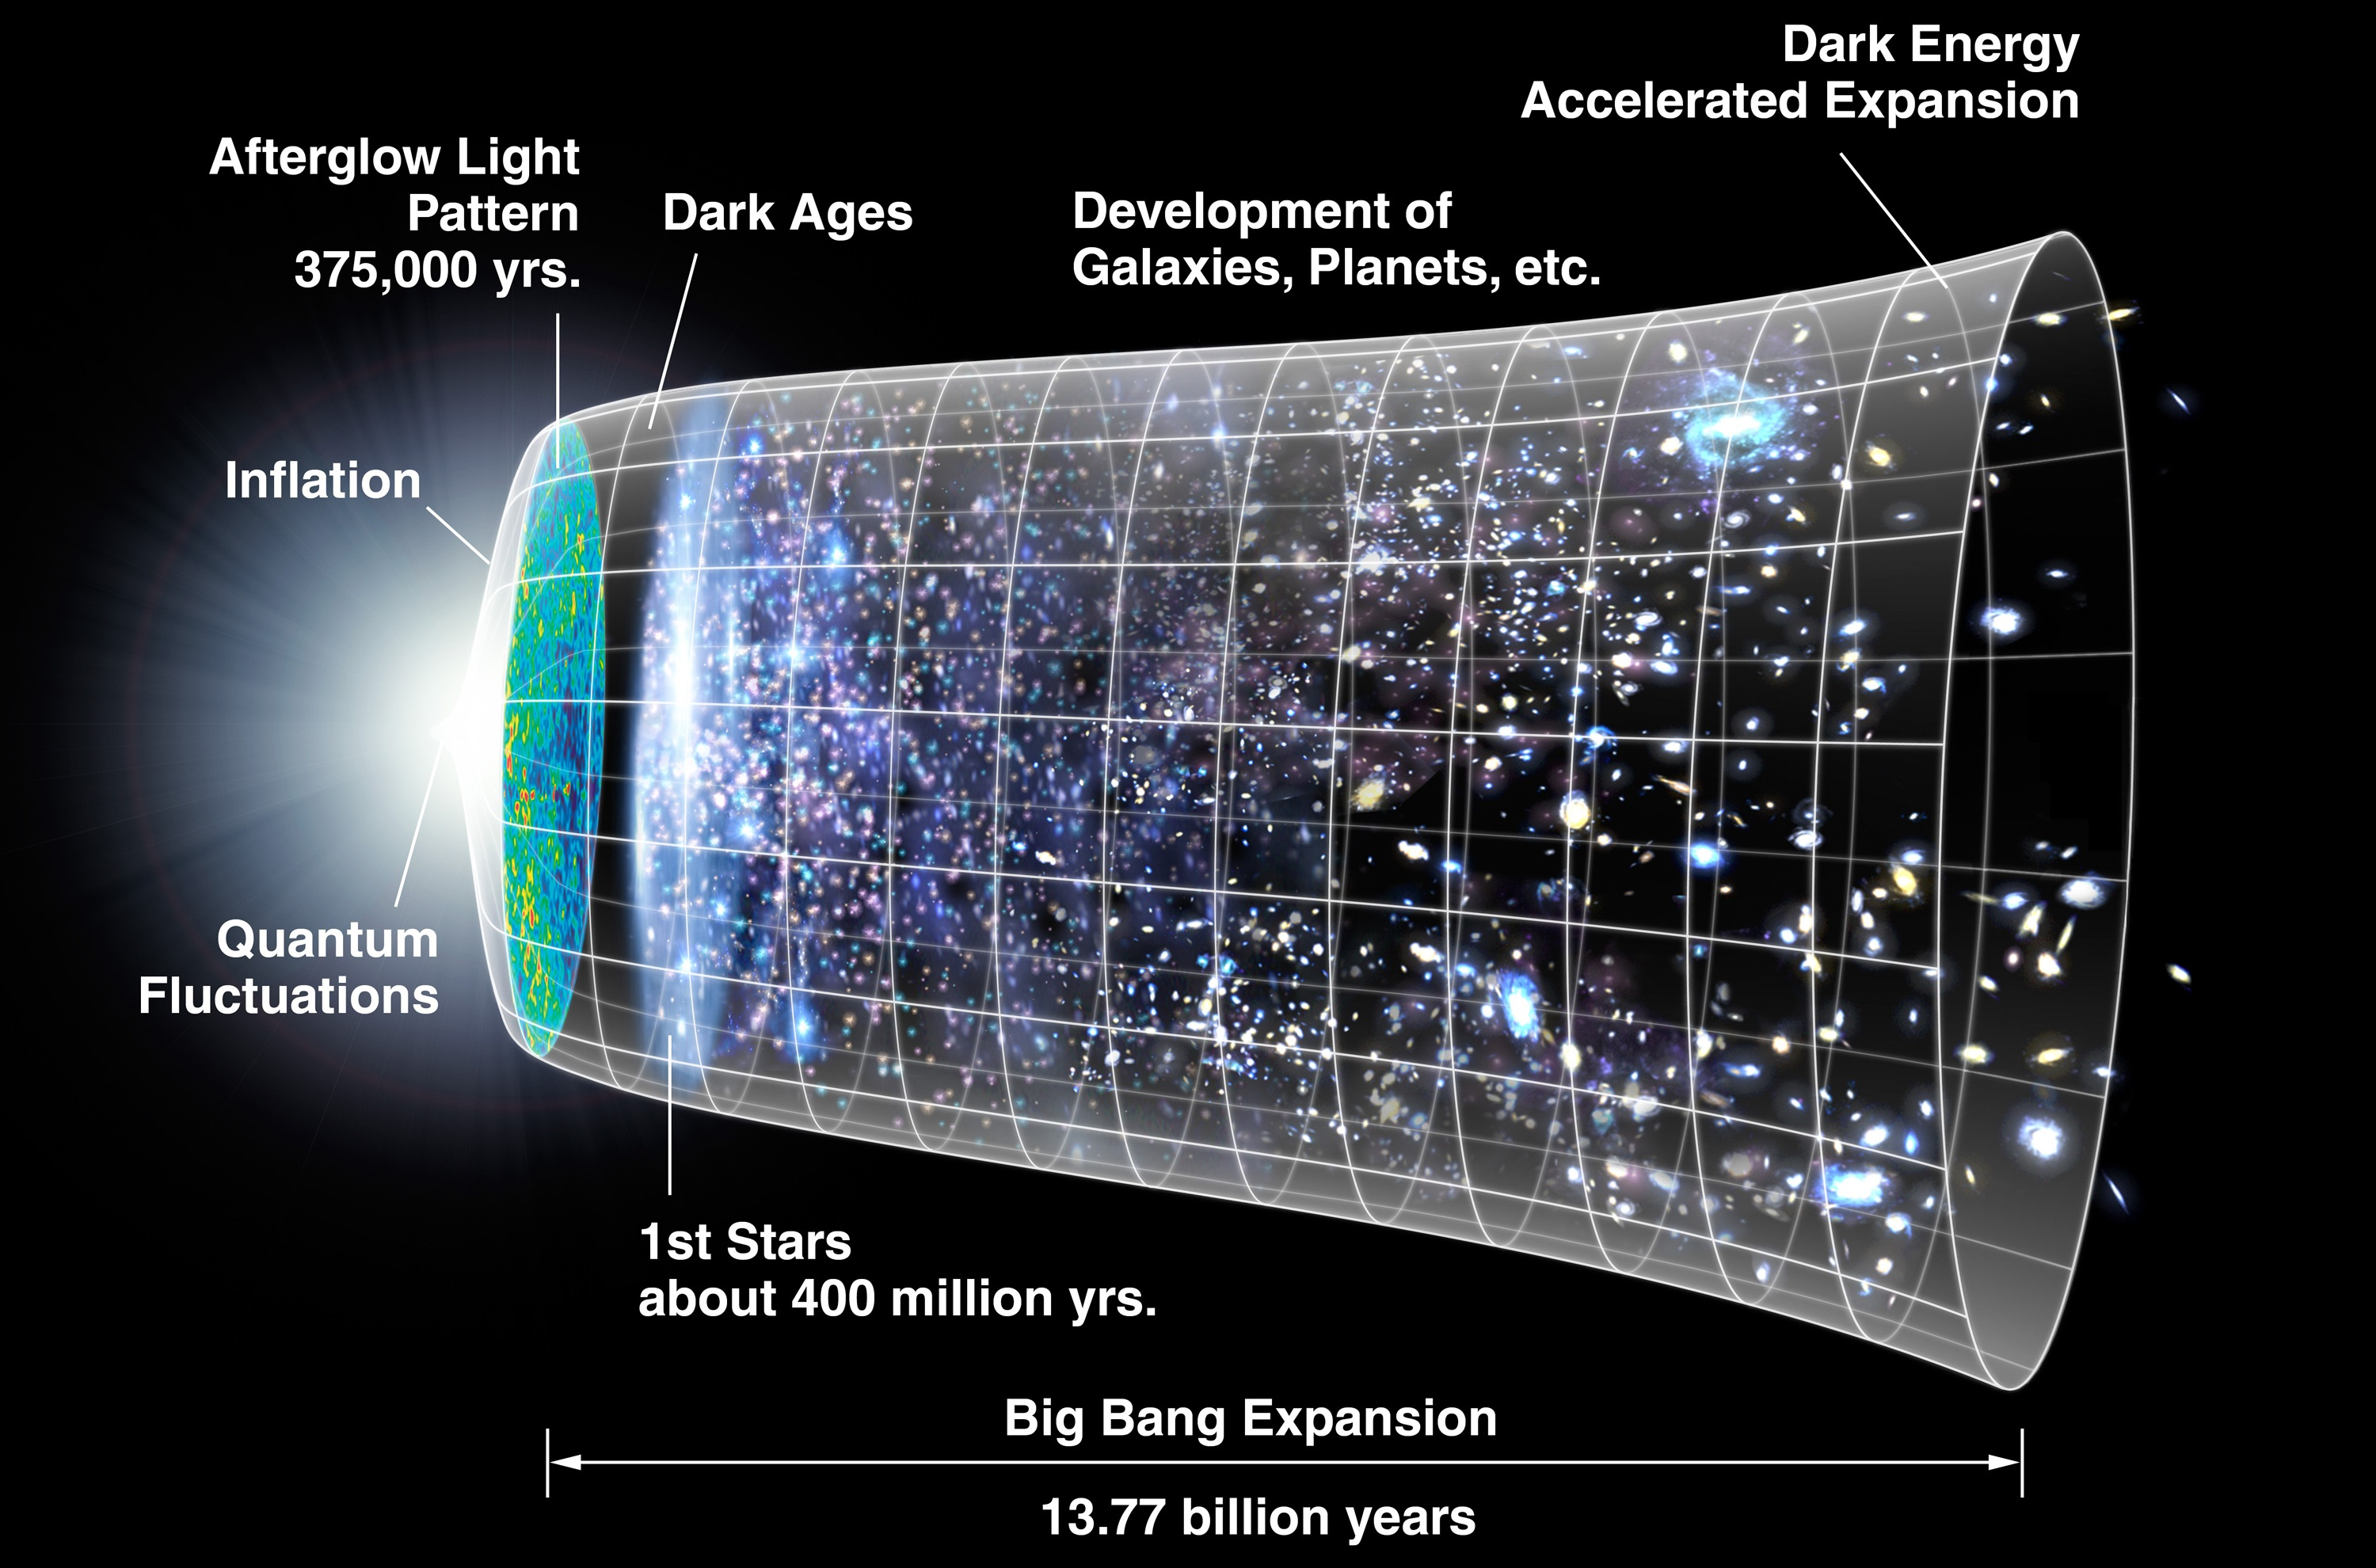
\includegraphics[width=12.5cm]{bigbang.jpg}
    \caption{\centering \footnotesize{Timeline of the expansion of the universe as per the Big Bang Theory (\textit{Time and Size not to Scale})} \protect\cite{bigbangpic}}
    \label{fig:bigbang}
\end{figure}

Matter, some atoms, formed \cite{hubblebigbang} and dominated over the antimatter \cite{britbigbang}.
Under the assumption that Albert Einstein's general theory of relativity correctly describes the relationship between matter and gravitational forces,
gravity brought matter into greater clumps that are known in the current day as our stars, planets, and galaxies
\cite{hubblebigbang}.

With the rapid expansion, the universe released a flood of radiation, alongside the matter, was also released into the new vast space
\cite{britbigbang,spacebigbang}
in the process known as "reheating", which is "the process whereby the inflation's energy density is converted back
into conventional matter after inflation
\cite{reheating}.
The radiation that was released then travelled through space, and the remnants of the early stages of the universe are known
as the cosmic microwave background (CMB) radiation \cite{britbigbang}, seen in figure \ref{fig:cmb}, 
though sometimes also referred to as the "'afterglow' of the Big Bang"
\cite{spacebigbang}.
These measurments are what allow scientists to predict the age of the universe relative to the currently measured rate of expansion of the universe
\cite{hubblebigbang}

\begin{figure} [H]
    \centering
    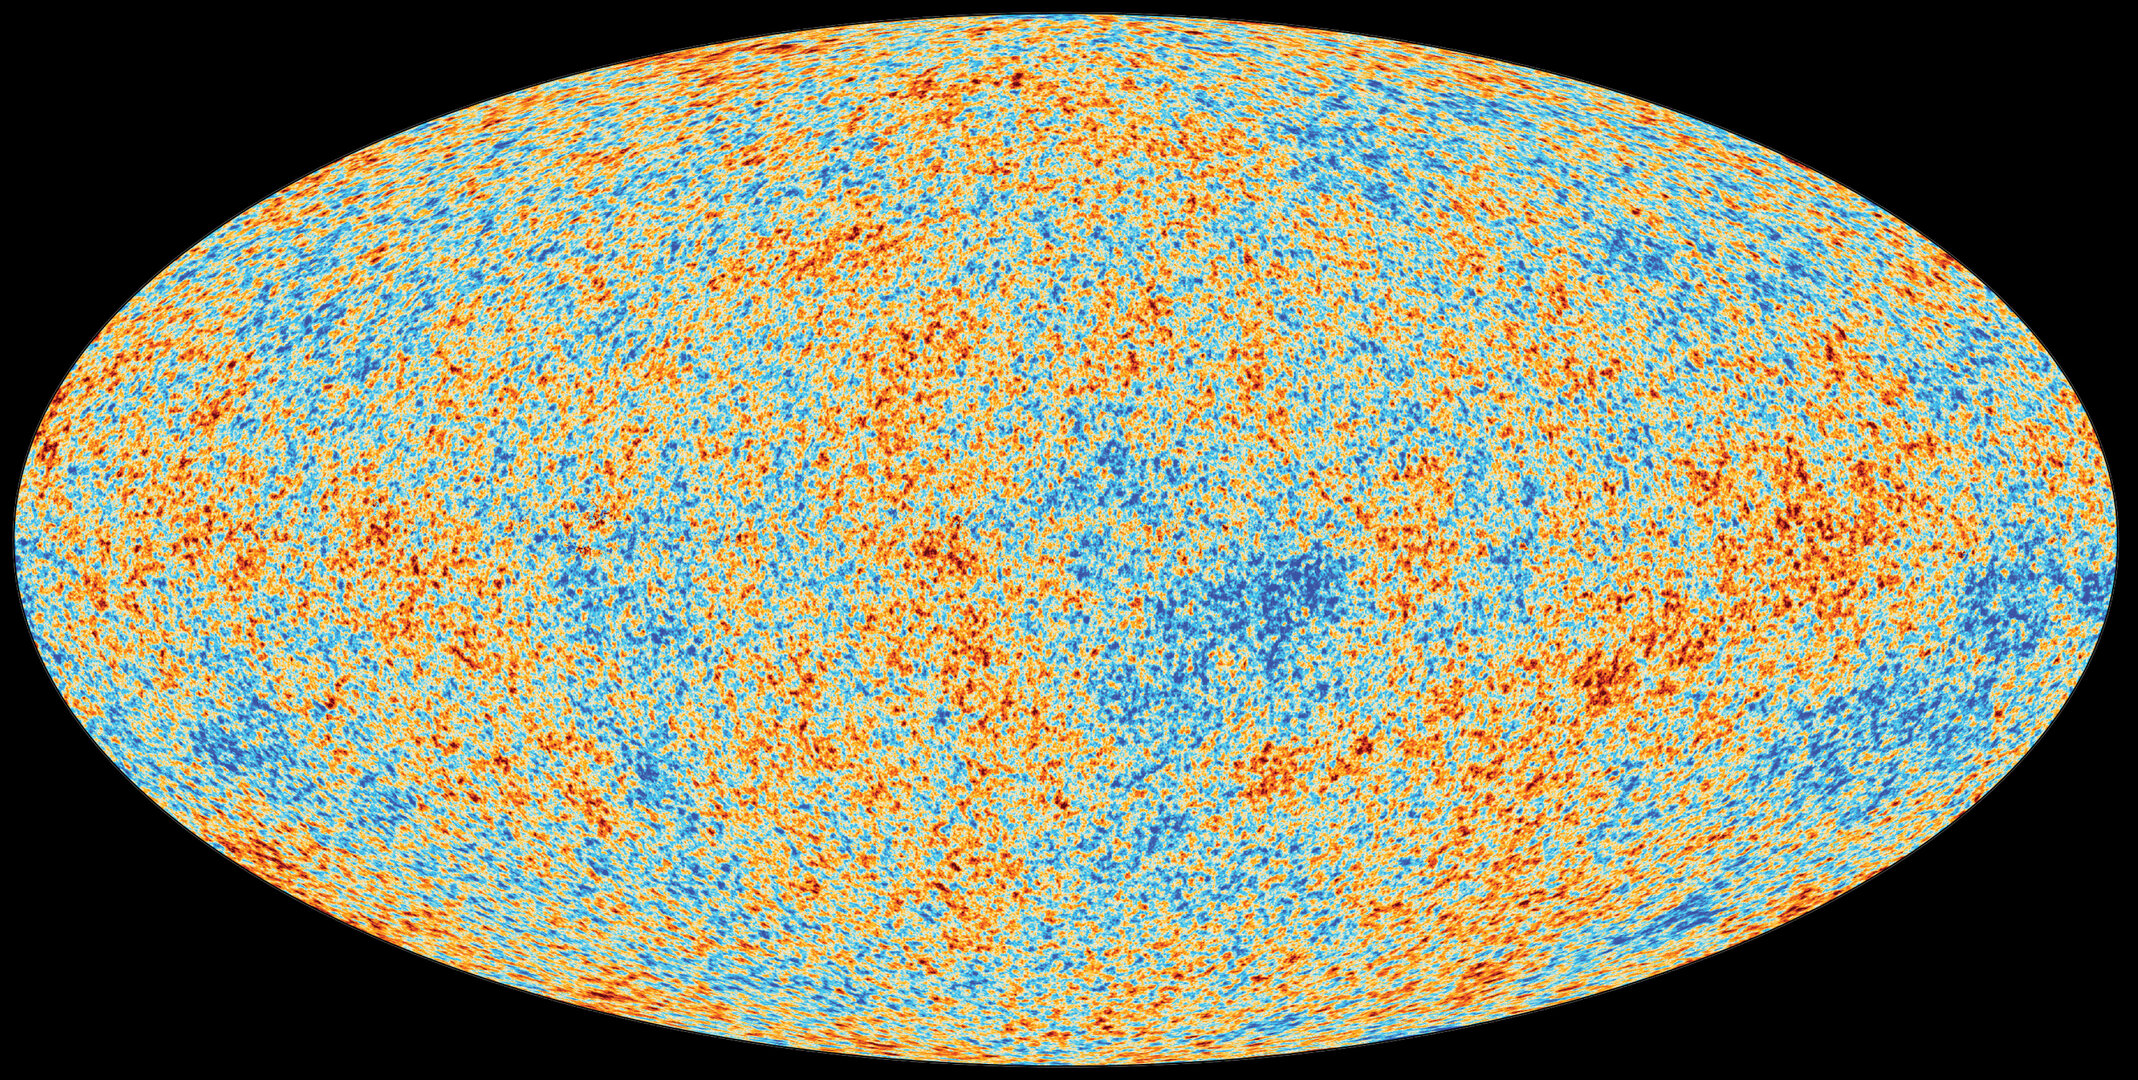
\includegraphics[width=12.5cm]{cmb.jpg}
    \caption{\centering \footnotesize{Cosmic Microwave Background (CMB) Radiation \protect\cite{cmbpic}}}
    \label{fig:cmb}
\end{figure}

\subsection{Spectrum, Spectrometry, Spectroscopy} \label{sec:1.2}

The electromagnetic spectrum describes all forms of electromagnetic radiation, including visible light, as it varies with wavelength
and frequency  
\cite{britspectra,hubblespectra}.
Spectroscopes are equipments used to visually observe the spectra and spectrographs photograph and map the studied spectra
\cite{britspectra}.
There are three main ways that the spectra can be classified, as illustrated in figure \ref{fig:spectra} \cite{spectrapic}:

\begin{itemize}
    \item \textbf{The continuous spectrum} contains all light emitted in a certain range from hot, dense light sources (like stars)
    from which the radiation travels out in all directions through space. The range of colours emitted depends on the temperature.
    \item \textbf{The absorption spectrum} is measured when light from a continuous source, like a star, passes through a cloud of cooler gas.
    The wavelengths that will be absorbed depend on the composition and elements of the gas, as well as its temperature and density. The wavelengths
    that didn't pass through are what appear as dark lines on the continuous spectrum known as the absorption line spectrum \cite{cosmosabsorp}.
    \item \textbf{The emmission spectrum} is measured when atoms become excited after light, like from a star, passes through a cloud of gas.
    The light can heat up the cloud of gas, thus exciting the atoms and causing them to release light. The light which the gas releases depends on the
    composition and elements, temperature, and density of the gas cloud. The light emitted will appear as coloured lines.
\end{itemize}

\textbf{Spectroscopy} studies the absorption and emission of light and matter radiation \cite{britspectrosco} and how matter would theoretically interact with radiation \cite{ataspectrosco}.
It provides the theoretical backbone to quantum research, particularly on the atomicc structure and radiation
\cite{ataspectrosco}.

\textbf{Spectrometry} puts quantitative values to the theory explored by spectroscopy by measuring the interactions between light (electromagnetic radiation)
and matter
\cite{ataspectrosco}.

\begin{figure}[H]
    \centering
    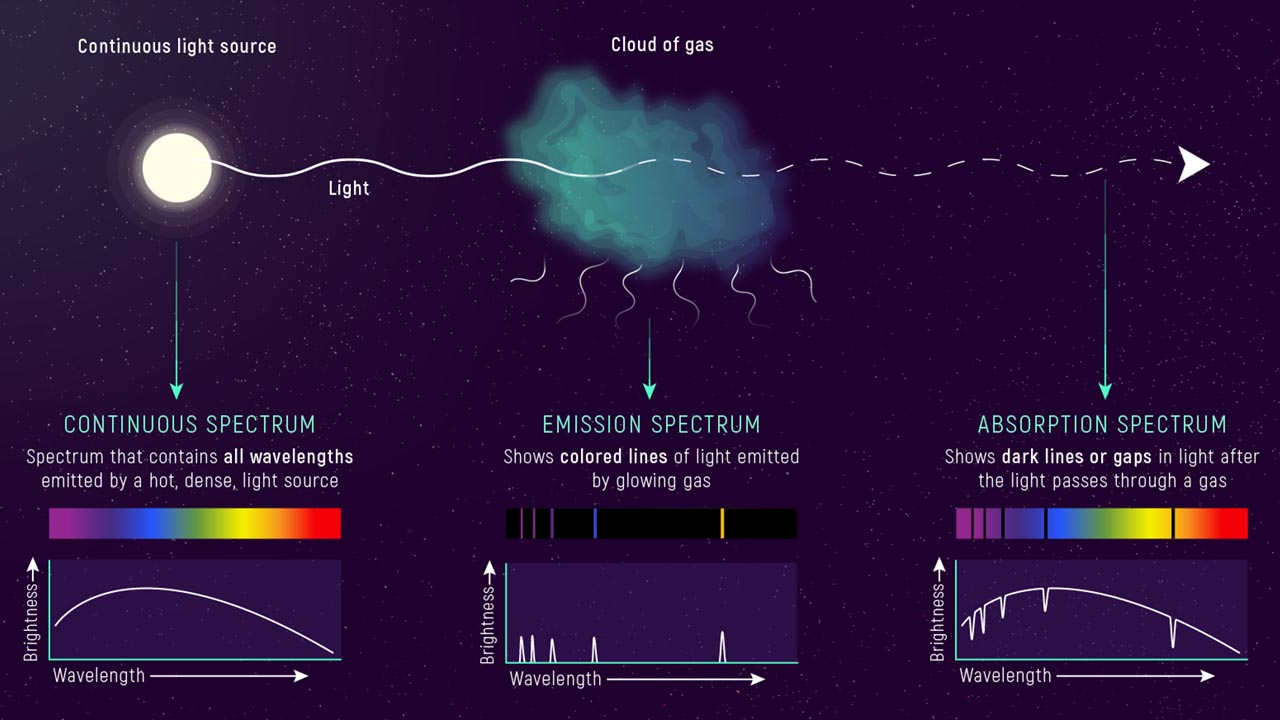
\includegraphics[width=15cm]{spectra.jpg}
    \caption{\centering \footnotesize{Types of spectra: continuous, emission, absorption \protect\cite{spectrapic}}}
    \label{fig:spectra}
\end{figure}

The understanding of electromagnetic spectra is essential in the sudy of the universe. Radio waves and microwaves have the lowest energies and longest wavelengths, as seen in
figure \ref{fig:wavelength}, which allows them to pierce dense stellar dust and gas clouds
\cite{hubblespectra}.
Infrared light can measure the molecular make-up of different stars and planets within our solar system.
The light seen emitted by majority of stars is within our visible light spectrum, which is quite narrow. Hotter stars have more energy and therefore shorter wavelengths
which makes them appear bluer in colour, whereas cooler stars have less energy and so longer wavelengths making them appear redder in colour
\cite{hubblespectra}.
Ultraviolet (UV) can be used to locate and identify the hottest (more energetic) stars as well as stellar nurseries.
X-rays and gamma rays, the most energetic light with the smallest wavelengths, are emitted mostly from materials around a black hole or from
the incredibly energetic and bright, and unstable, neutron stars
\cite{hubblespectra}.

\begin{figure}[H]
    \centering
    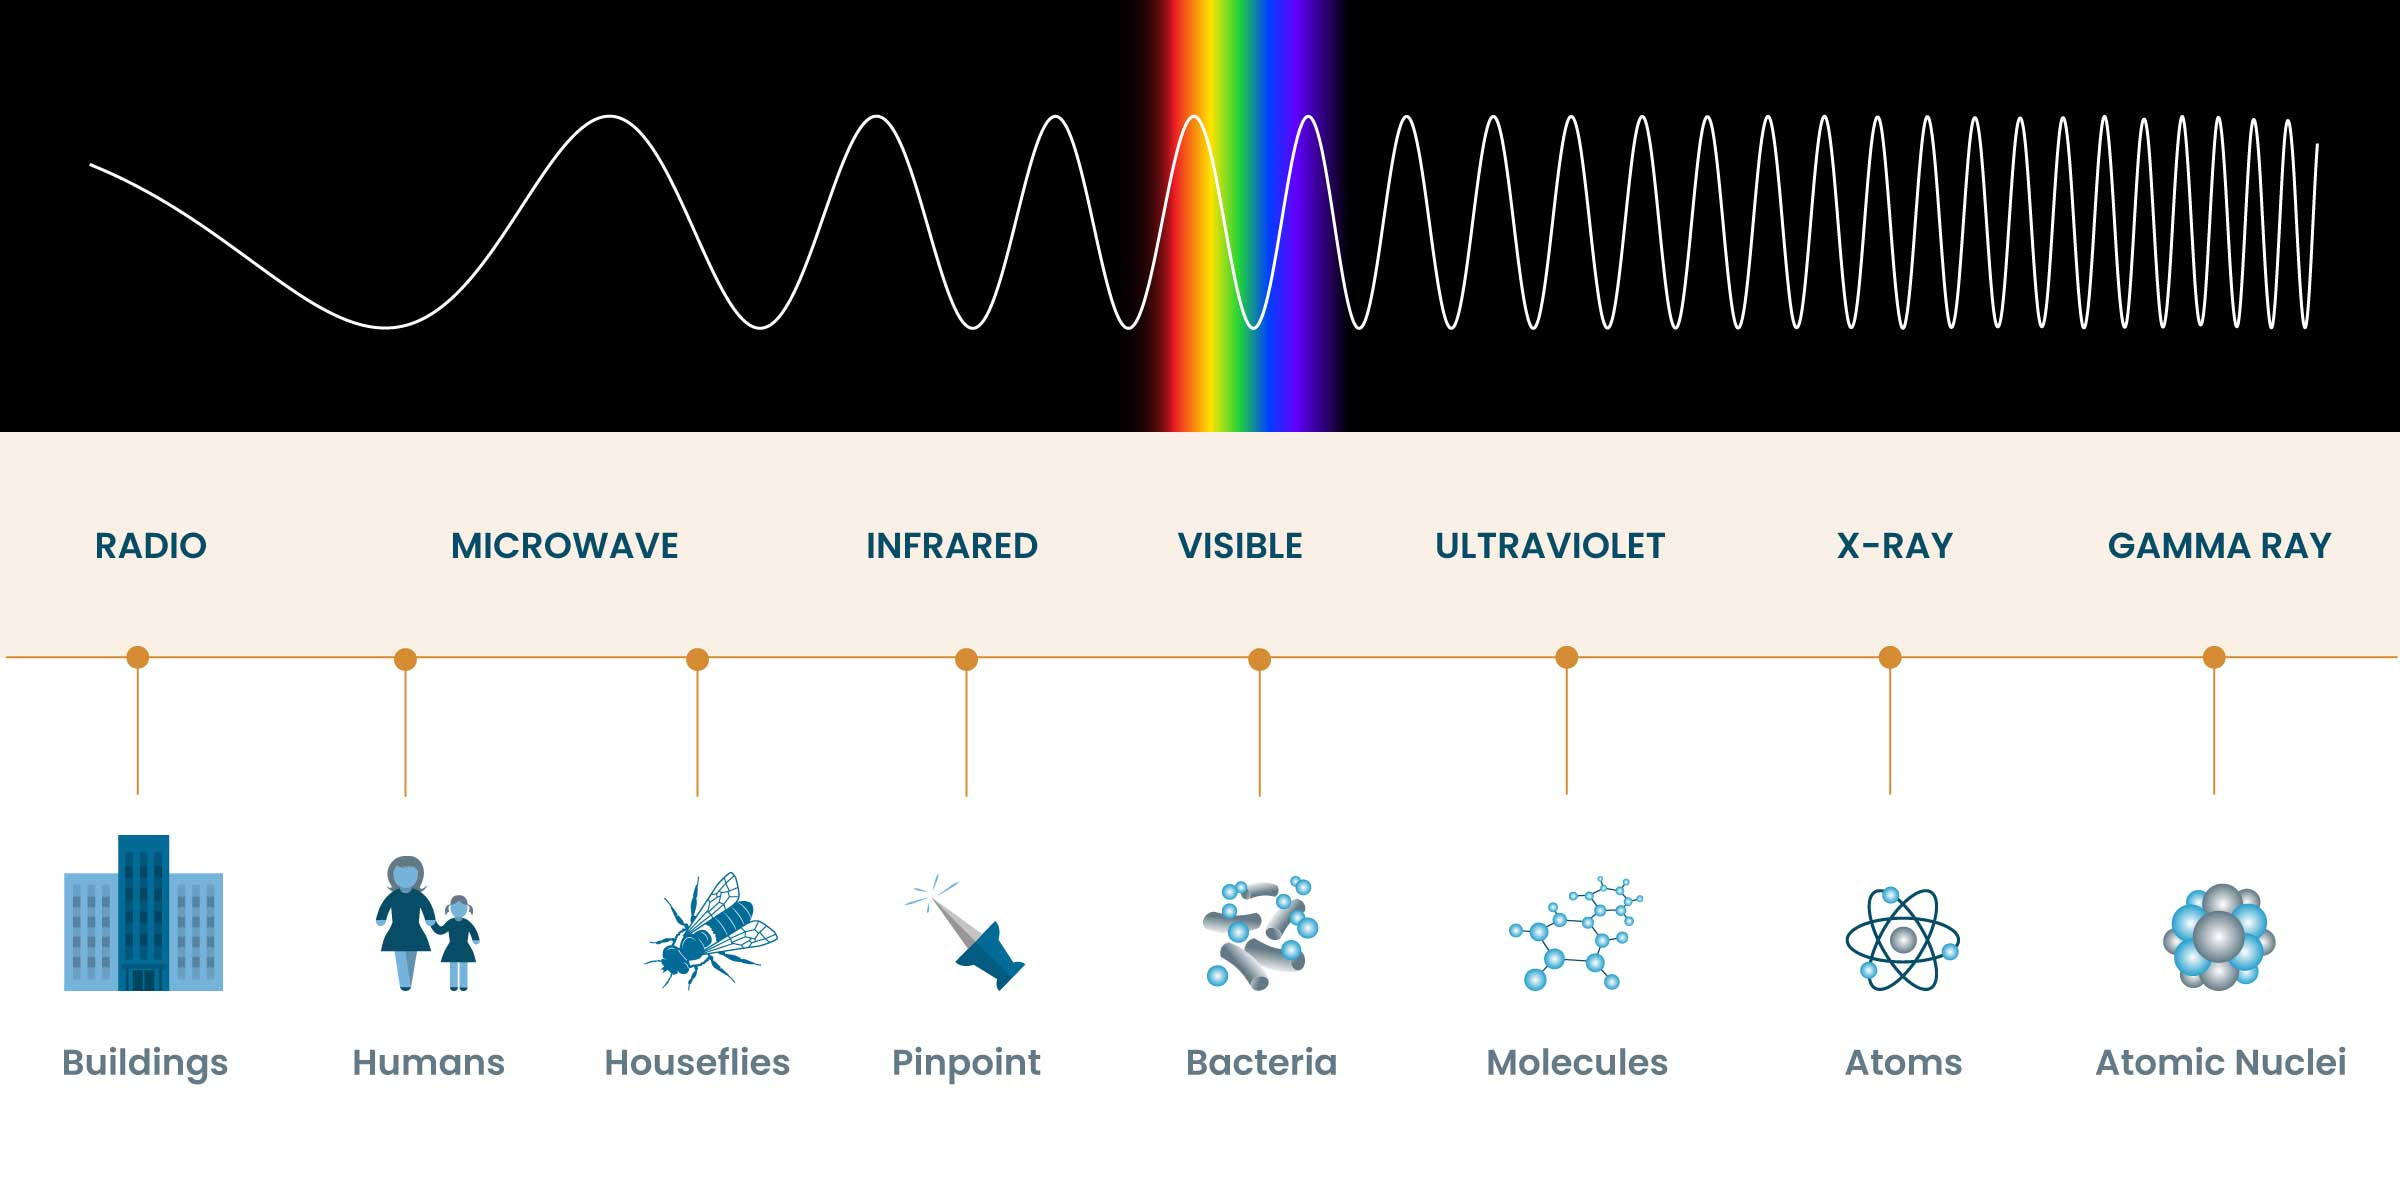
\includegraphics[width=15cm]{light waves.jpg}
    \caption{\centering \footnotesize{Comparison of different types of light, including wavelength size, and frequency \protect\cite{hubblespectra}}}
    \label{fig:wavelength}
\end{figure}

\vspace{1cm}

\subsubsection{Apparent and Absolute Magnitude} \label{sec:1.2.1}

Magnitude is a measure of the brightness of a star or other celestial body. The brighter the object, the lower the magnitude
\cite{britmag}.
The magnitude of the celestial objects are divided into two types of observation:

\begin{itemize}
    \item \textbf{Apparent magnitude, m,} is used to describe how bright a celestial object appears from the view on Earth. Some of the brightest objects we can see,
    like our Sun and planets, have \textit{negative} apparent magnitude values (Sun = -26.7, Pluto (at brightest) = +13.7, for reference)
    \cite{lcomag}.
    \item \textbf{Absolute magnitude, M,} is defined as the magnitude of the star if the distance between it and Earth were 10 parsecs (pc)
    \cite{lcoabsmag,cosmosabsmag}.
    When at a set distance, astronomers are then able to compare intrinsic brightness of stars. The absolute magnitude refers to the absolute 'visual' magnitude, which restricts
    the measurement of the brightness to wavelength (4000 - 7000 Å)
    \cite{cosmosabsmag}.
\end{itemize}

\begin{figure}[H]
    \centering
    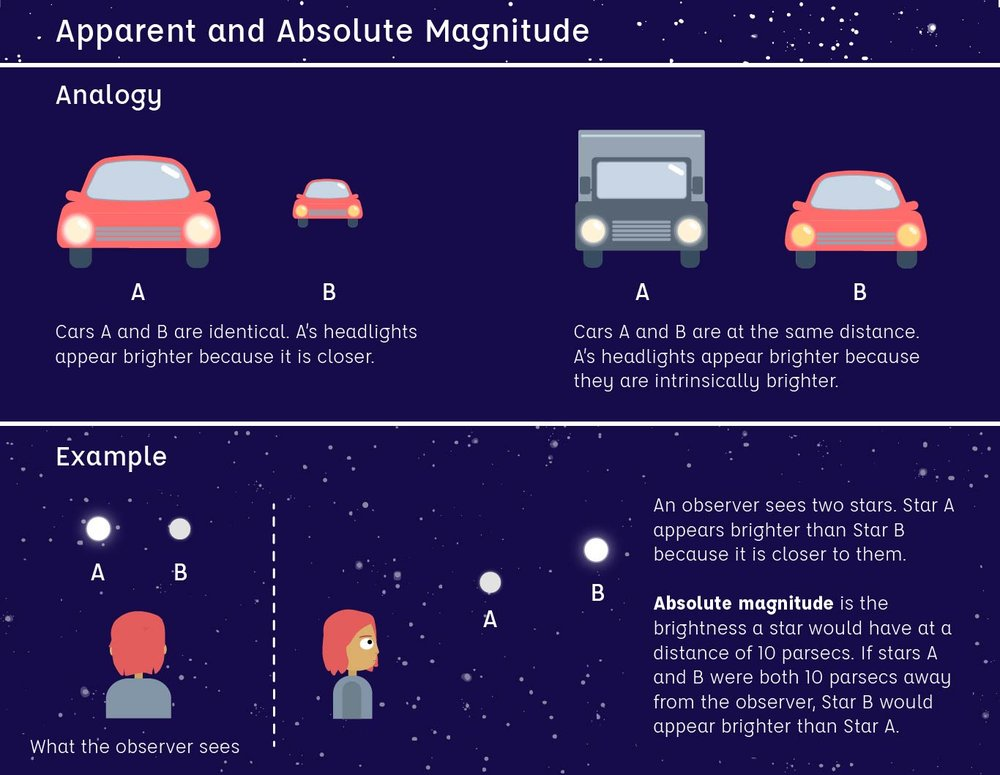
\includegraphics[width=15cm]{lcomag.jpg}
    \caption{\centering \footnotesize{Absolute and apparent magnitude as real life examples \protect\cite{lcoabsmag} \textit{(Illustrated by Alice Hopkinson)}}}
    \label{fig:absappmag}
\end{figure}

Absolute (\textbf{M}) and apparent (\textbf{m}) magnitudes can be used using equation \ref{eq:1} with \textbf{D} as the distance in parsecs (pc). The magnitude does not have a unit.
The distance modulus is $m - M$
\cite{cosmosabsmag}.

\begin{gather} \label{eq:1}
    M = m + 5 - 5 (\log_{10} D) \quad , \quad m - M = 5 \log_{10} \left( \frac{D}{10} \right)
\end{gather}

The above equation (\ref{eq:1}) can be manipulated to find the distance, \textbf{D}:

\begin{gather} \label{eq:2}
    \log_{10}D = \frac{m - M + 5}{5} \quad \implies \quad D = 10^{\frac{m - M + 5}{5}}
\end{gather}

\vspace{0.5cm}

\subsubsection{H and K Lines} \label{sec:1.2.2}

The Fraunhofer lines are the dark lines in absorption spectroscopy obtained from a star and the selective absorption of radiation at those specific wavelengths
by the gases in their atmospheres, as covered in §\ref{sec:1.2}
\cite{brithk}.

\begin{figure}[H]
    \centering
    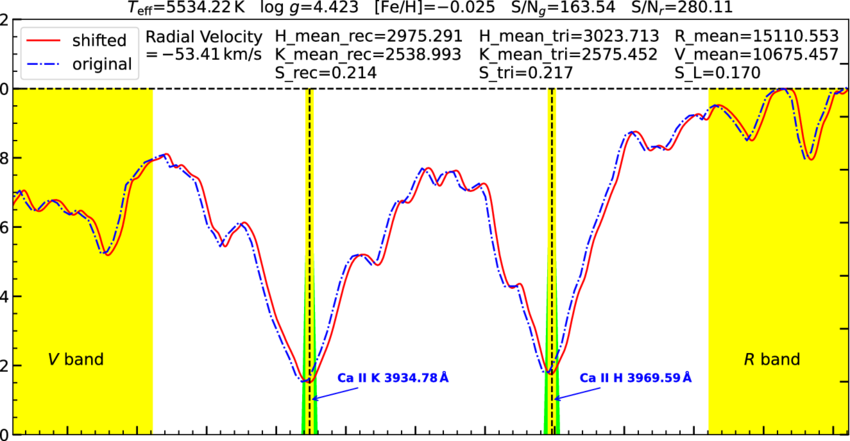
\includegraphics[width=15cm]{handklines.png}
    \caption{\centering \footnotesize{An example of the spectrum diagrams of Ca II H and K lines \protect\cite{rgatehk}}}
    \label{fig:hklines}
\end{figure}

The Ca II (ionized calcium) H and K lines, at \textbf{3968.469 Å} and \textbf{3933.663 Å} respectively, are the two strongest lines in the visible solar spectrum
\cite{UCDhubble,aandahk}, clearly labelled as the vertical dotted lines in figure \ref{fig:hklines}.
These Fraunhofer lines can be used not only for determining redshift but also for the stellar classifications of stars
\cite{britstar}.

With measured wavelengths of the H and K lines compared against the accepted values \break (\textbf{3968.469 Å} and \textbf{3933.663 Å} respectively) in equations \ref{eq:3} and \ref{eq:5}
the velocity at which these wavelengths are being redshifted (§\ref{sec:1.2.3}) can then be calculated with equations \ref{eq:4} and \ref{eq:6}, the Doppler shift formula.

\begin{minipage}{0.45\textwidth}
    \begin{gather} \label{eq:3}
        \Delta \lambda_H = \lambda_{H \: measured} - \lambda_H 
    \end{gather}
    \vspace{-1.5em}
    \begin{gather} \label{eq:4}
        v_H = c \left( \frac{\Delta \lambda_H}{\lambda_H} \right)
    \end{gather}
\end{minipage}
\hfill
\begin{minipage}{0.45\textwidth}
    \begin{gather} \label{eq:5}
        \Delta \lambda_K = \lambda_{K \: measured} - \lambda_K 
    \end{gather}
    \vspace{-1.5em}
    \begin{gather} \label{eq:6}
        v_K = c \left( \frac{\Delta \lambda_K}{\lambda_K} \right)
    \end{gather}
\end{minipage}

\subsubsection{What is 'Redshift'?} \label{sec:1.2.3}

Redshift is a fundamental concept that explains the continuous expansion of the universe.
It can be interpreted literally as the wavelength of a source being stretched as it moves away, similar to how the wavelength would compress if it were moving towards the viewer (blueshift)
\cite{esaredshift,earthskyredshift}.
As the wavelength stretches, from what was covered in §\ref{sec:1.2}, the colour of the light shifts redder
\cite{esaredshift}.
These are the basic principles of the 'Doppler Effect', which also applies to sound waves
\cite{esaredshift,lcoredshift,britredshift,earthskyredshift}.

It was the scientist Edwin Hubble that reported and named this curiosity after witnessing a distant galaxy receding from the Milky Way system in 1929, hence the 
'Hubble Parameter' covered in §\ref{sec:1.3}
\cite{britredshift}.

This does not mean, however, that the galaxies themselves are moving but rather the fabric of space itself is expanding
\cite{esaredshift}.
In figure \ref{fig:redshift} it is seen how the absorption lines (covered in §\ref{sec:1.2}) shift in colour further up and into the red part
of the electromagnetic spectrum, hence the 'redshift'
\cite{earthskyredshift}.

\begin{figure}[H]
    \centering
    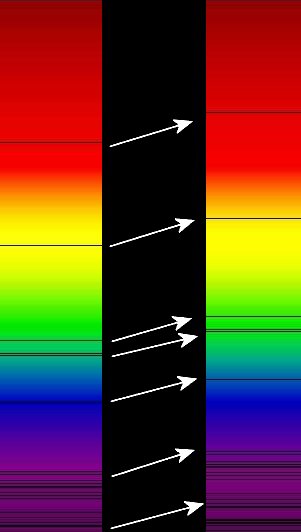
\includegraphics[width=5cm]{Redshift.png}
    \caption{\centering \footnotesize{The dark absorption lines of a star at rest (\textit{left}) get shifted towards red if the star is moving away from Earth (\textit{right}) \protect\cite{earthskyredshift} (via Wikipedia)}}
    \label{fig:redshift}
\end{figure}

Redshift can be observed even in the early stages of the universe's expansion with the CMB radiation seen in figure \ref{fig:cmb}, §\ref{sec:1.1.1}.

\vspace{1cm}

\subsection{The Hubble Parameter} \label{sec:1.3}

The Hubble cosntant, or Hubble parameter, $H_0$, is the measurement of the velocity at which a celestial object at a given distance is moving away from the viewer,
as was discussed in §\ref{sec:1.1}
\cite{brithubble,chicagohubble}.

The true value of the Hubble constant is still left up to debate even in the modern day. Hubble's original value for $H_0$ was $500 \: km/s/Mpc$,
but modern interpretations of this constant vary at much smaller values
\cite{brithubble,chicagohubble}.
These modern values tend to range between $67$ km/s/Mpc and around $74$ km/s/Mpc
\cite{chicagohubble,nasahubble}, the range of these values can be obsereved in figure \ref{fig:hubble}

The Hubble parameter can be calculated using equation \ref{eq:7}, wher \textbf{H} is the Hubble parameter in $km/s/Mpc$, \textbf{v} is the velocity
of the H or K line that was measured (equation \ref{eq:3}, \ref{eq:5}), and \textbf{D} is the distance for the respective H and K lines measured (equation \ref{eq:4}, \ref{eq:6}).

\begin{gather} \label{eq:7}
    H = \frac{v}{D}
\end{gather}

\begin{figure}[H]
    \centering
    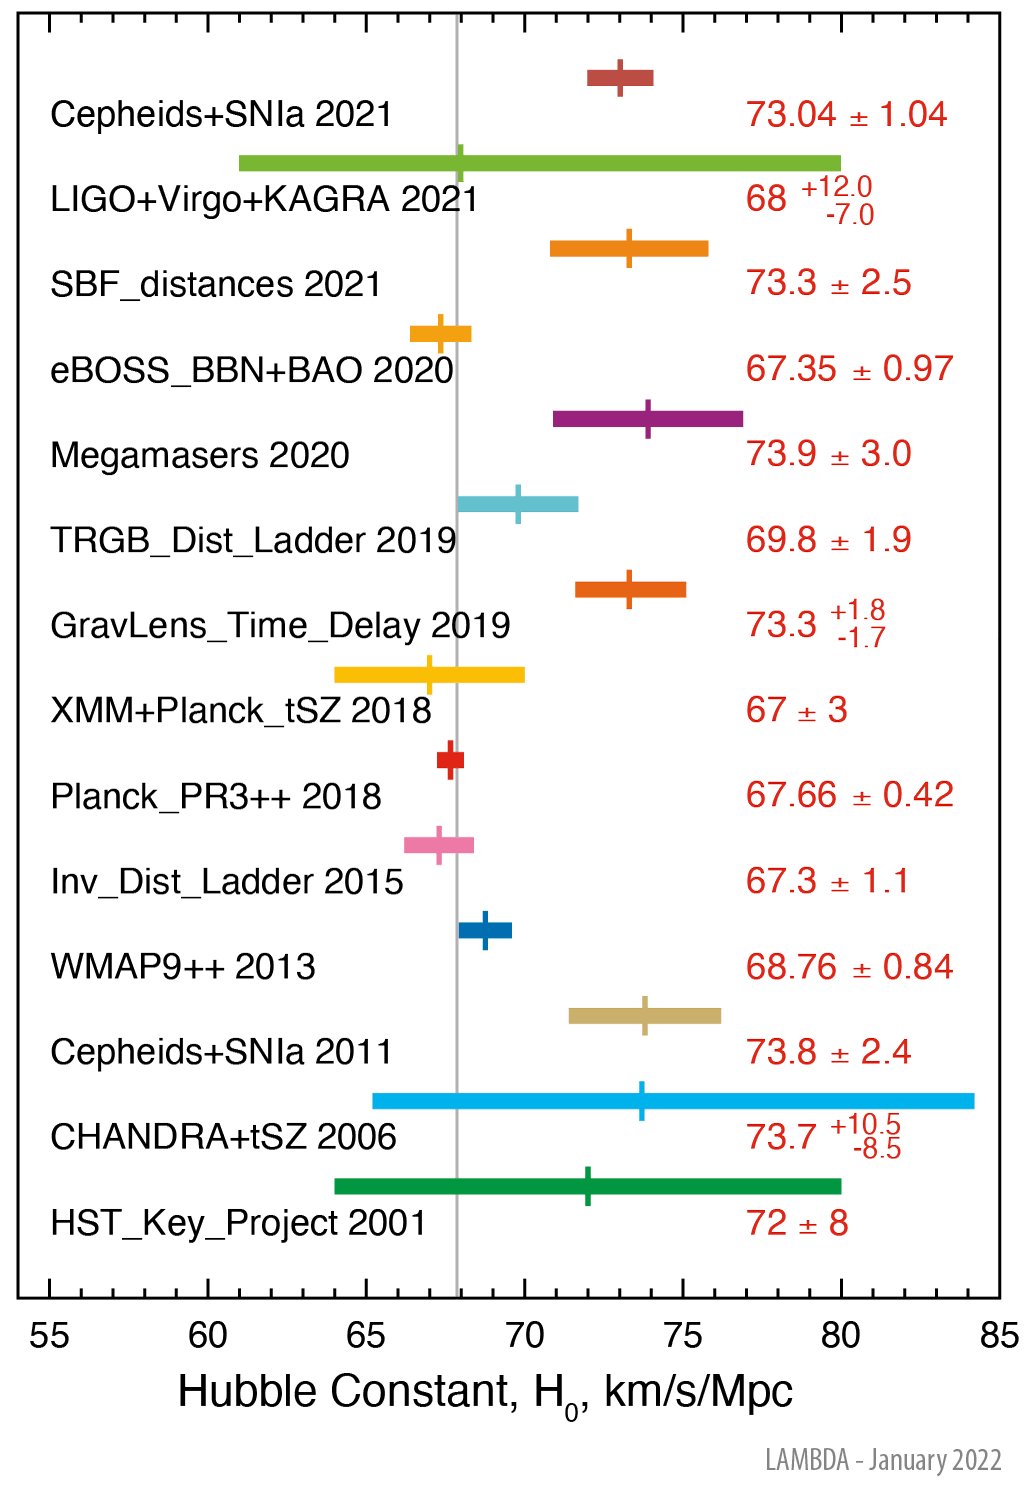
\includegraphics[width=8cm]{hubble constant nasa.png}
    \caption{\centering \footnotesize{'The Hubble Constant $H_O$ characterizes the present-day expansion rate of the universe' \protect\cite{nasahubble}}}
    \label{fig:hubble}
\end{figure}

\section{Methodology} 

This experiment made use of the \textit{Contemporary Laboratory Experience in Astronomy}, CLEA, software and the \textit{Hubble Redshift Distance Relation} program included in the package.
CLEA is an online software developed to simulate and illustrate modern astronomical techniques in a 'real' night sky
\cite{clea}.
Different sizes and locations of the telescopes are offered, but the default is set to the KPNO 0.9m (36") telescope in Kitt Peak National Observatory, Arizona.
The program does a good job at simulating the 'realness' of using a telescope as the stars move against the dark night sky with the Earth's rotation. The 'tracking'
button available removes the uncertainty of movement while measuring.

The software program used for this experiment offers 6 fields with simulated galaxies that can be measured. These fields are:

\begin{itemize}
    \item Ursa Major I
    \item Ursa Major II
    \item Coma Berenices
    \item Bootes
    \item Corona Borealis
    \item Saggitarius, which features the faces of some famous physicists as galaxies that can be observed.
\end{itemize}

Data about different galaxies in each seperate field was gathered with the use of the 'instrument view', the spectrometer, available that allows for the collection of the different
wavelengths to then be classified. Brighter galaxies released more light so they were quicker to read as it would gather more photons in less time. The longer
the spectrometer is collecting photons for, the less noise will be present in the spectrum and therefore correctly locating the peaks of the Ca II H and K lines (§\ref{sec:1.2.2}) would be easier.

\begin{figure}[H]
    \centering
    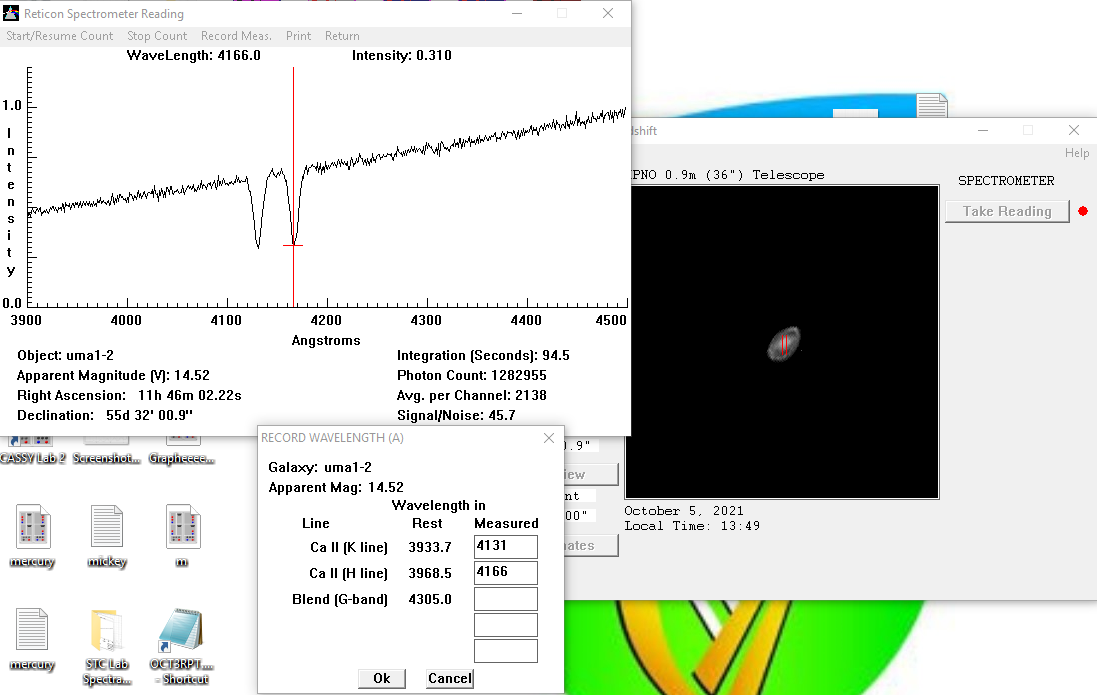
\includegraphics[width=15cm]{URSA1 program.png}
    \caption{\centering \footnotesize{Screenshot of the program running}}
    \label{fig:program}
\end{figure}

The amount that galaxy had redshifted can be observed before being explicitly calculated by observing how much it has deviated from the expected values discussed in §\ref{sec:1.2.2}.
The more redshifted the lines are, the faster that galaxy is travelling away from Earth (§\ref{sec:1.2.3}).

The list of data collected for each galaxy includes:

\begin{itemize}
    \item \textbf{Object name:} the name provided for the galaxy being observed.
    \item \textbf{Apparent magnitude:} the brightness as it appears from Earth (§\ref{sec:1.2.1}).
    \item \textbf{Photon count:} the number of photons absorbed in the time of observation.
    \item \textbf{Ca II (K line):} the left-most absorption line, in Ångstroms.
    \item \textbf{Ca II (H line):} the next absorption line, in Ångstroms.
    \item \textbf{Blend (G-band):} an outlier absorption line, classified as bright spots in stars that contain CH (methylidyne) molecules \cite{gband}, in Ångstroms.
\end{itemize}

The uncertainties for the measured wavelengths were no more than $\pm 3$ Å for every galaxy.

\newpage

\section{Results and Calculations} \label{sec:3}

Below, in table \ref{tab:1}, are the values gathered with the use of the CLEA program. The wavelengths are converted to kilometres (km) to aid 
in later calculations. G-band excluded for the purpose of calculations, but can be found in the Appendix, table \ref{tab:A1}.

\vspace{0.5cm}

\renewcommand{\arraystretch}{1.3}

\begin{table}[H]

    \centering
    \resizebox{\textwidth}{!}{
    
        \begin{tabular}{|c|c|c|c|c|c|}
        \hline
        \begin{tabular}[c]{@{}c@{}}Object\\ Name\end{tabular} & \begin{tabular}[c]{@{}c@{}}Apparent\\ Magnitude\end{tabular} & \begin{tabular}[c]{@{}c@{}}Ca II\\ (K-line) (Å)\end{tabular} & \begin{tabular}[c]{@{}c@{}}$\lambda_K$\\ (K-line) (km) $\: \times \: 10^{-10}$ \end{tabular} & \begin{tabular}[c]{@{}c@{}}Ca II\\ (H-line) (Å)\end{tabular} & \begin{tabular}[c]{@{}c@{}}$\lambda_H$\\ (H-line) (km) $\: \times \: 10^{-10}$\end{tabular} \\
        \hline
        \textbf{uma1-2}                                       & $14.52$                                                      & $4131.0 \: \pm \: 2$                                         & $(4.131 \: \pm \: 0.002)$                                                                    & $4166.0 \: \pm \: 2$                                         & $(4.166 \: \pm \: 0.002)$                                                                   \\
        \hline
        \textbf{uma1-3}                                       & $14.49$                                                      & $4130.0 \: \pm \: 2$                                         & $(4.130 \: \pm \: 0.002)$                                                                    & $4167.0 \: \pm \: 2$                                         & $(4.167 \: \pm \: 0.002)$                                                                   \\
        \hline
        \textbf{uma2-1}                                       & $16.87$                                                      & $4484.0 \: \pm \: 1$                                         & $(4.484 \: \pm \: 0.001)$                                                                    & -                                                            & -                                                                                           \\
        \hline
        \textbf{uma2-3}                                       & $16.89$                                                      & $4484.0 \: \pm \: 1$                                         & $(4.484 \: \pm \: 0.001)$                                                                    & -                                                            & -                                                                                           \\
        \hline
        \textbf{Coma2}                                        & $12.55$                                                      & $4012.0 \: \pm \: 1$                                         & $(4.012 \: \pm \: 0.001)$                                                                    & $4048.0 \: \pm \: 1$                                         & $(4.048 \: \pm \: 0.001)$                                                                   \\
        \hline
        \textbf{Coma3}                                        & $12.45$                                                      & $4012.0 \: \pm \: 1$                                         & $(4.012 \: \pm \: 0.001)$                                                                    & $4047.0 \: \pm \: 1$                                         & $(4.047 \: \pm \: 0.001)$                                                                   \\
        \hline   
        \textbf{Boot2}                                        & $16.76$                                                      & $4445.0 \: \pm \: 2$                                         & $(4.445 \: \pm \: 0.002)$                                                                    & $4485.0 \: \pm \: 2$                                         & $(4.485 \: \pm \: 0.002)$                                                                   \\
        \hline
        \textbf{Boot3}                                        & $16.72$                                                      & $4445.0 \: \pm \: 2$                                         & $(4.445 \: \pm \: 0.002)$                                                                    & $4484.0 \: \pm \: 2$                                         & $(4.484 \: \pm \: 0.002)$                                                                   \\
        \hline
        \textbf{CrBor1}                                       & $15.08$                                                      & $4209.0 \: \pm \: 2$                                         & $(4.209 \: \pm \: 0.002)$                                                                    & $4247.0 \: \pm \: 2$                                         & $(4.247 \: \pm \: 0.002)$                                                                   \\
        \hline
        \textbf{CrBor3}                                       & $15.35$                                                      & $4209.0 \: \pm \: 2$                                         & $(4.209 \: \pm \: 0.002)$                                                                    & $4246.0 \: \pm \: 2$                                         & $(4.246 \: \pm \: 0.002)$                                                                   \\
        \hline
        \textbf{LAM}                                          & $11.15$                                                      & $3973.0 \: \pm \: 2$                                         & $(3.973 \: \pm \: 0.002)$                                                                    & $4008.0 \: \pm \: 2$                                         & $(4.008 \: \pm \: 0.002)$                                                                   \\
        \hline
        \textbf{RFG}                                          & $12.31$                                                      & $4012.0 \: \pm \: 2$                                         & $(4.012 \: \pm \: 0.002)$                                                                    & $4048.0 \: \pm \: 2$                                         & $(4.048 \: \pm \: 0.002)$                                                                   \\
        \hline
        \end{tabular}

    }
    
    \caption{\centering \footnotesize{Results collected from the CLEA \textit{Hubble Redshift Distance Relation} simulator from each field:}}
    \footnotesize{Ursa Major I: 'uma1-', Ursa Major II: 'uma2-', Coma Berenices: 'Coma', Bootes: 'Boot', Corona Borealis: 'CrBor', Saggitarius: 'ABC'.}
    \label{tab:1}

\end{table}

\vspace{1.5cm}

\subsection{Determining the Hubble's Parameter} \label{sec:3.1}

To determine Hubble's parameter prior calculations must be made using the formulas disccused in §\ref{sec:1}. Equation \ref{eq:2} is used to calculate the distance in mega parsecs (Mpc).
Equations \ref{eq:3} and \ref{eq:5} are then used to find the redshift in the H- and K-lines, the difference between the accepted and measured values.
Equations \ref{eq:4} and \ref{eq:6} calculate the velocities of the H- and K-lines and the average between both is found where applicable (Ursa Major II values are the exception).

\begin{table}[H]
    
    \centering
    \resizebox{\textwidth}{!}{

        \begin{tabular}{|c|c|c|c|c|c|c|c|}
        \hline
        \begin{tabular}[c]{@{}c@{}}Object\\ Name\end{tabular} & \begin{tabular}[c]{@{}c@{}}Absolute\\ Magnitude\end{tabular} & \begin{tabular}[c]{@{}c@{}}Distance\\ (Mpc)\end{tabular} & \begin{tabular}[c]{@{}c@{}}$\Delta \lambda_K$\\ (km)\end{tabular} & \begin{tabular}[c]{@{}c@{}}$\Delta \lambda_H$\\ (km)\end{tabular} & \begin{tabular}[c]{@{}c@{}}Velocity\\ (K-line) (km/s)\end{tabular} & \begin{tabular}[c]{@{}c@{}}Velocity\\ (H-line) (km/s)\end{tabular} & \begin{tabular}[c]{@{}c@{}}Velocity\\ Average (km/s)\end{tabular} \\ \hline
        \textbf{uma1-2}                                       & -22                                                          & 201.4                                                    & $1.373 \: \times \: 10^{-11}$                                     & $1.975 \: \times \: 10^{-11}$                                     & $1.0313 \: \times \: 10^{4}$                                       & $1.4930 \: \times \: 10^{4}$                                       & $1.2622 \: \times \: 10^{4}$                                      \\ \hline
        \textbf{uma1-3}                                       & -22                                                          & 198.6                                                    & $1.363 \: \times \: 10^{-11}$                                     & $1.985 \: times \: 10^{-11}$                                      & $1.02386 \: \times \: 10^{4}$                                      & $1.5006 \: \times \: 10^{4}$                                       & $1.2622 \: \times \: 10^{4}$                                      \\ \hline
        \textbf{uma2-1}                                       & -22                                                          & 594.3                                                    & $4.903 \: \times \: 10^{-11}$                                     & -                                                                 & $3.6831 \: \times \: 10^{4}$                                       & -                                                                  & $3.6831 \: \times \: 10^{4}$                                      \\ \hline
        \textbf{uma2-3}                                       & -22                                                          & 599.8                                                    & $4.903 \: \times \: 10^{-11}$                                     & -                                                                 & $3.6831 \: \times \: 10^{4}$                                       & -                                                                  & $3.6831 \: \times \: 10^{4}$                                      \\ \hline
        \textbf{Coma2}                                        & -22                                                          & 81.3                                                     & $1.830 \: \times \: 10^{-12}$                                     & $7.950 \: \times \: 10^{-12}$                                     & $1.3747 \: \times \: 10^{3}$                                       & $6.0098 \: \times \: 10^{3}$                                       & $3.6922 \: \times \: 10^{3}$                                      \\ \hline
        \textbf{Coma3}                                        & -22                                                          & 77.6                                                     & $1.830 \: \times \: 10^{-12}$                                     & $7.850 \: \times \: 10^{-12}$                                     & $1.3747 \: \times \: 10^{3}$                                       & $5.9343 \: \times \: 10^{3}$                                       & $3.6544 \: \times \: 10^{3}$                                      \\ \hline
        \textbf{Boot2}                                        & -22                                                          & 564.9                                                    & $4.513 \: \times \: 10^{-11}$                                     & $5.165 \: \times \: 10^{-11}$                                     & $3.3901 \: \times \: 10^{4}$                                       & $3.9045 \: \times \: 10^{4}$                                       & $3.6473 \: \times \: 10^{4}$                                      \\ \hline
        \textbf{Boot3}                                        & -22                                                          & 554.6                                                    & $4.513 \: \times \: 10^{-11}$                                     & $5.155 \: \times \: 10^{-11}$                                     & $3.3901 \: \times \: 10^{4}$                                       & $3.8969 \: \times \: 10^{4}$                                       & $3.6435 \: \times \: 10^{4}$                                      \\ \hline
        \textbf{CrBor1}                                       & -22                                                          & 260.6                                                    & $2.513 \: \times \: 10^{-11}$                                     & $2.785 \: \times \: 10^{-11}$                                     & $1.6173 \: \times \: 10^{4}$                                       & $2.1053 \: \times \: 10^{4}$                                       & $1.8613 \: \times \: 10^{4}$                                      \\ \hline
        \textbf{CrBor3}                                       & -22                                                          & 295.1                                                    & $2.513 \: \times \: 10^{-11}$                                     & $2.775 \: \times \: 10^{-11}$                                     & $1.6173 \: \times \: 10^{4}$                                       & $2.0978 \: \times \: 10^{4}$                                       & $1.8575 \: \times \: 10^{4}$                                      \\ \hline
        \textbf{LAM}                                          & -22                                                          & 42.7                                                     & $-2.070 \: \times \: 10^{-12}$                                    & $3.950 \: \times \: 10^{-12}$                                     & $-1.5549 \: \times \: 10^{3}$                                      & $2.9860 \: \times \: 10^{3}$                                       & $7.1553 \: \times \: 10^{2}$                                      \\ \hline
        \textbf{RFG}                                          & -22                                                          & 72.8                                                     & $1.830 \: \times \: 10^{-12}$                                     & $7.950 \: \times \: 10^{-12}$                                     & $1.3747 \: \times \: 10^{3}$                                       & $6.0098 \: \times \: 10^{3}$                                       & $3.6922 \: \times \: 10^{3}$                                      \\ \hline
        \end{tabular}

    }

    \caption{\centering \footnotesize{Results calculated from the values gathered in table \protect\ref{tab:1} for each field:}}
    \footnotesize{Ursa Major I: 'uma1-', Ursa Major II: 'uma2-', Coma Berenices: 'Coma', Bootes: 'Boot', Corona Borealis: 'CrBor', Saggitarius: 'ABC'.}
    \label{tab:2}

\end{table}

The values calculated in table \ref{tab:2} can then be plotted on graph with the (average) velocities (km/s) calculated on the y-axis and the distances (Mpc) calculated
on the x-axis. By the slope of the line of best fit the average Hubble parameter can then be found.

\begin{figure}[H]
    \centering
    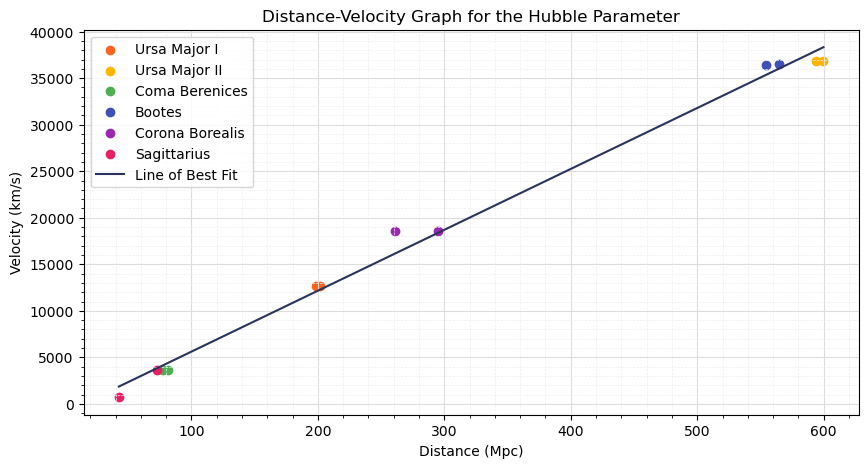
\includegraphics[width=\textwidth]{HUBBLEgraph.png}
    \caption{\centering \footnotesize{The distance-velocity graph of the measurements taken in tables \protect\ref{tab:1} and \protect\ref{tab:2} with each field measurement clearly colour differentiated.}}
    \label{fig:graph}
\end{figure}

The slope of the graph (figure \ref{fig:graph}) was found to be \textbf{65.45}, which can be taken as the average value of the Hubble parameter.

\newpage

\subsection{Determining the Age of the Universe} \label{sec:3.2}

Using the average value of the Hubble parameter found in §\ref{sec:3.1} and equation \ref{eq:7} discussed in §\ref{sec:1.3}, the velocity of
a theoretical galaxy \textbf{800 Mpc} away can be found:

\begin{gather} \label{eq:8}
    v \: = \: HD \: = \: (65.45)(800) \: = \: 52 \: 360 \: km/s
\end{gather}

So the velocity at which this theoretical galaxy is being redshifted by would be \textbf{52 360 km/s}. This answer can be confirmed by looking at where this value is on
the line of best fit in the figure \ref{fig:extend} below.

\begin{figure}[H]
    \centering
    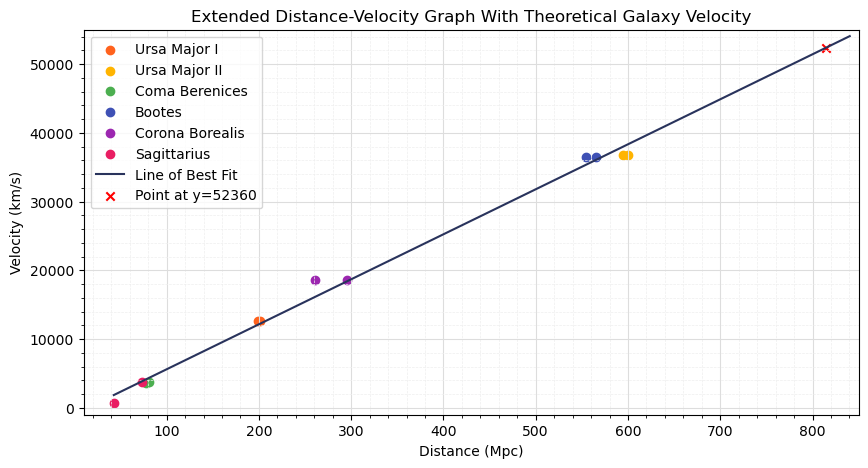
\includegraphics[width=\textwidth]{extended x.png}
    \caption{\centering \footnotesize{Extended axes and line of best fit to confirm the answer found in equation \protect\ref{eq:8}}}
    \label{fig:extend}
\end{figure}

It is also possible find how \textit{long ago} the universe started with this answer. 800 Mpc is $2.469 \: \times \: 10^{22}$ km. Using the time-distance-velocity relation,
this time can be calculated:

\begin{gather} \label{eq:9}
    T \: = \: \frac{D}{R} \: = \: \frac{2.469 \: \times \: 10^{22}}{52360} \: = \: 4.7154 \: \times \: 10^{17} s
\end{gather}

Therefore, from the values found in this experiment, the universe began $4.7154 \: \times \: 10^{17}$ s ago, which is about $1.4953 \: \times \: 10^{10}$ years ago, or 14.95 billion years ago!

\newpage

\section{Conclusion} \label{sec:4}

By the values found and calculated in §\ref{sec:3} it can be concluded that the experiment was successful in determining a Hubble parameter, \textbf{65.45 km/s/Mpc} that is consistent with the modern
values found for it, and that the age of the universe calculated, \textbf{14.95 billion years}, also aligns closely with the theoretical age.

In future renditions of this experiment the spectrometer could be allowed to run for longer to allow the collection of more photons in order
to reduce the amount of noise in the spectrograph, which would make reding the peaks for the H- and K-lines easier and would allow for the results ti be more accurate.
The bigger telescope options that are offered, such as the 4m Mayall telescope, could be used for the faster and more efficient collection of photons.

\newpage

%%%%%%%%%%%%%%%%%%%%%%%%%%%%%%%%%%%

\bibliographystyle{IEEEtran}
\bibliography{References}

\newpage

\section*{Appendix} \label{sec:A}
\addcontentsline{toc}{section}{Appendix}

\listoffigures

\listoftables

\subsection*{Raw Data}
\addcontentsline{toc}{subsection}{Raw Data}

\begin{table}[H]

    \centering

        \begin{tabular}{|c|c|c|}
        \hline
        \begin{tabular}[c]{@{}c@{}}Object\\ Name\end{tabular} & \begin{tabular}[c]{@{}c@{}}Photon\\ Count\end{tabular} & \begin{tabular}[c]{@{}c@{}}G-band\\ (Å)\end{tabular} \\ \hline
        \textbf{uma1-2}                                       & 1 282 955                                              & -                                                    \\ \hline
        \textbf{uma1-3}                                       & 698 783                                                & -                                                    \\ \hline
        \textbf{uma2-1}                                       & 505 811                                                & -                                                    \\ \hline
        \textbf{uma2-3}                                       & 211 690                                                & -                                                    \\ \hline
        \textbf{Coma2}                                        & 4 485 991                                              & $4391.0 \: \pm \: 1$                                 \\ \hline
        \textbf{Coma3}                                        & 7 819 425                                              & $4391.0 \: \pm \: 1$                                 \\ \hline
        \textbf{Boot2}                                        & 388 805                                                & -                                                    \\ \hline
        \textbf{Boot3}                                        & 604 865                                                & -                                                    \\ \hline
        \textbf{CrBor1}                                       & 614 332                                                & -                                                    \\ \hline
        \textbf{CrBor3}                                       & 1 741 655                                              & -                                                    \\ \hline
        \textbf{LAM}                                          & 8 762 232                                              & $4348.0 \: \pm \: 2$                                 \\ \hline
        \textbf{RFG}                                          & 6 031 871                                              & $4391.0 \: \pm \: 2$                                 \\ \hline
        \end{tabular}

    \caption{\centering \footnotesize{Table of the missing collected values from CLEA, photon count and G-band wavelengths}}
    \footnotesize{Ursa Major I: 'uma1-', Ursa Major II: 'uma2-', Coma Berenices: 'Coma', Bootes: 'Boot', Corona Borealis: 'CrBor', Saggitarius: 'ABC'.}
    \label{tab:A1}
    
\end{table}

\subsection*{Code}
\addcontentsline{toc}{subsection}{Code}

\begin{figure}[H]
    \centering
    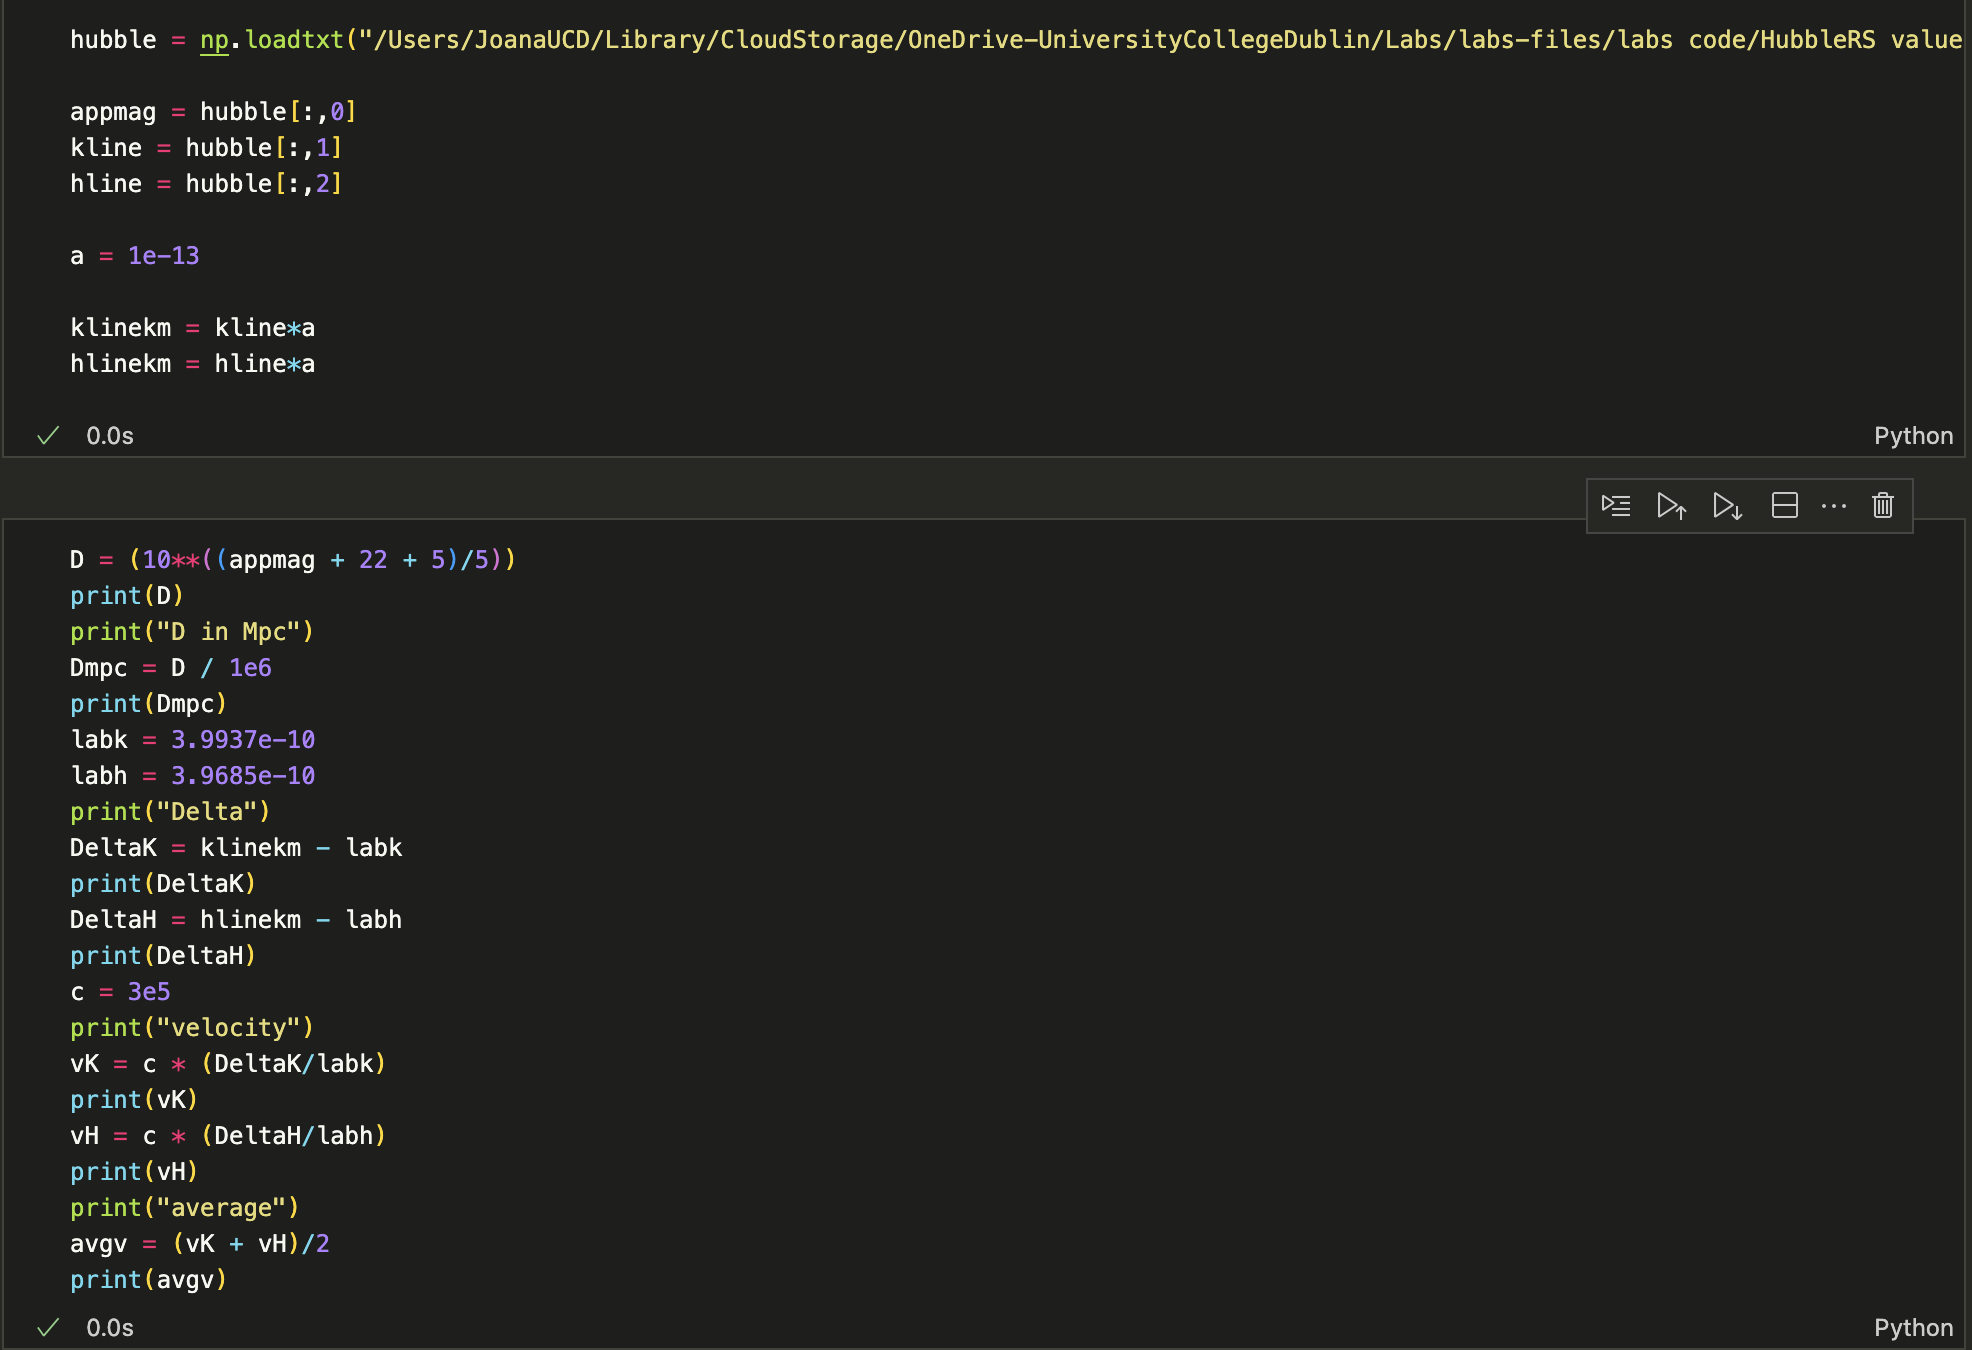
\includegraphics[width=14cm]{codeHUBBLE1.png}
    \caption{\centering Code for calculations (Python)}
    \label{fig:code1}  
\end{figure}

\newpage

\begin{figure}[H]
    \centering
    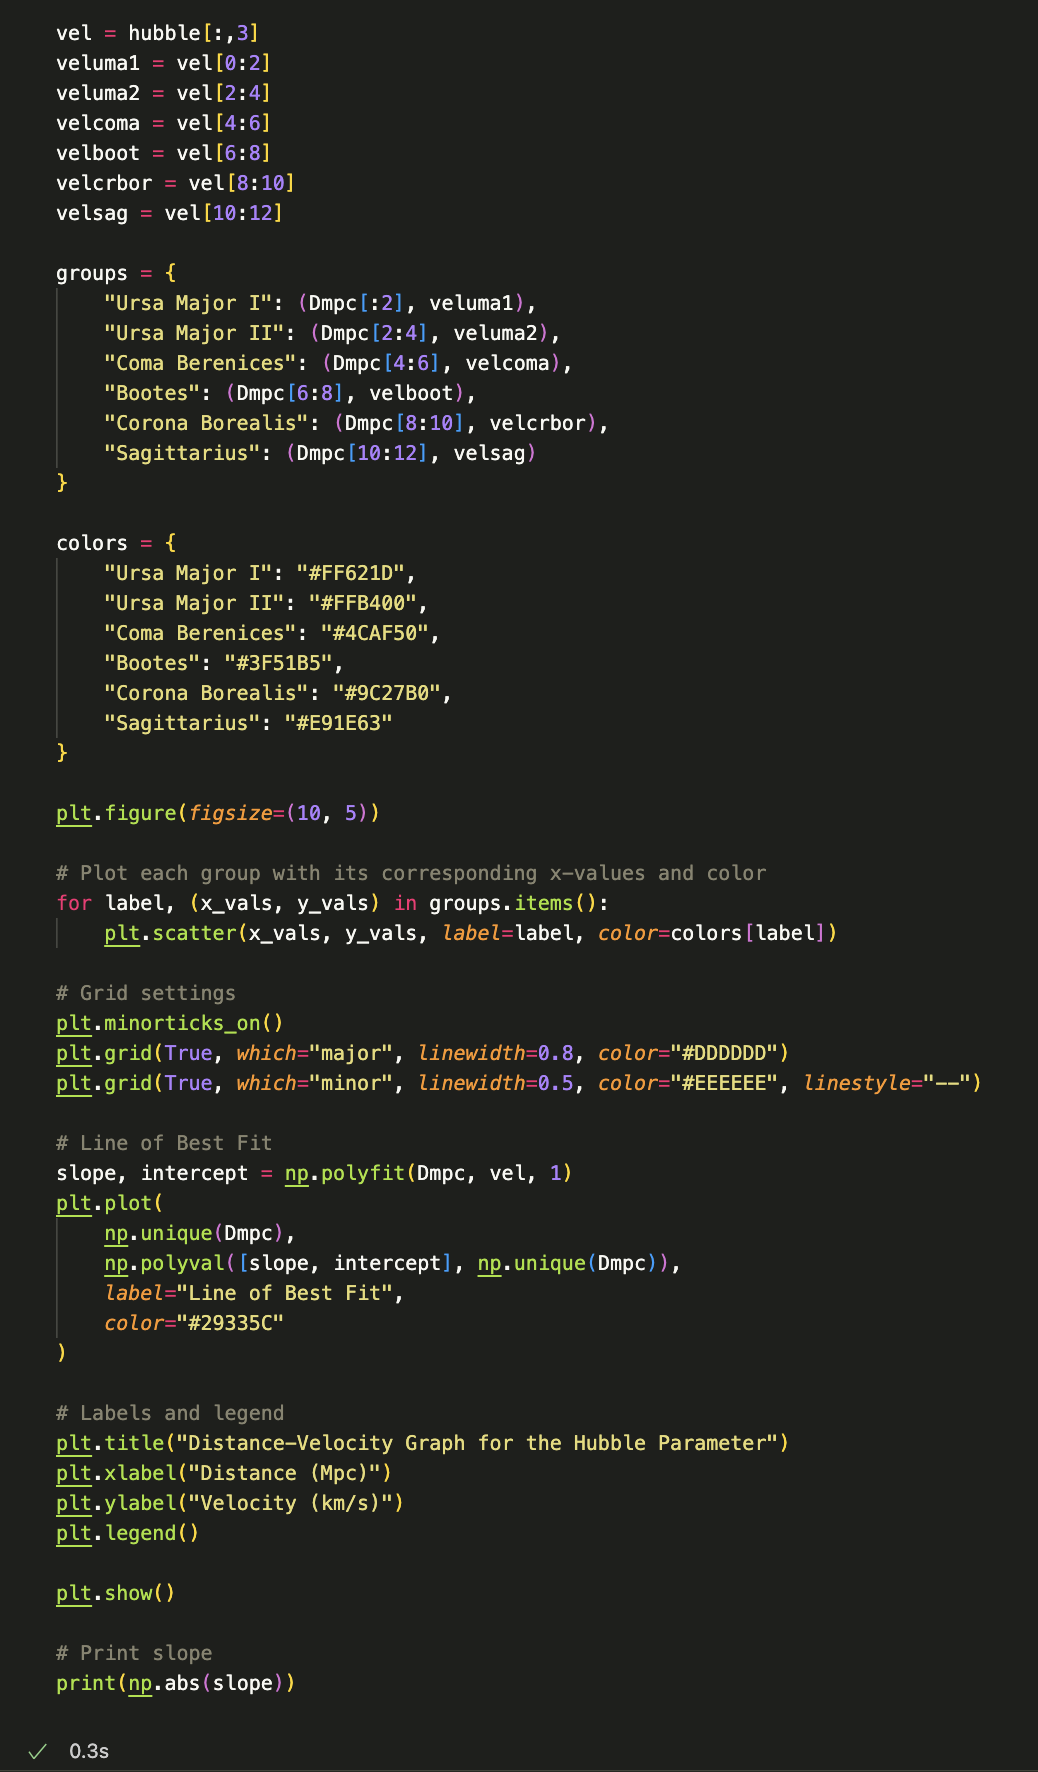
\includegraphics[width=14cm]{HUBBLEcode2.png}
    \caption{\centering Code for calculations (Python) Cont'd}
    \label{fig:code2}  
\end{figure}

\newpage

\begin{figure}[H]
    \centering
    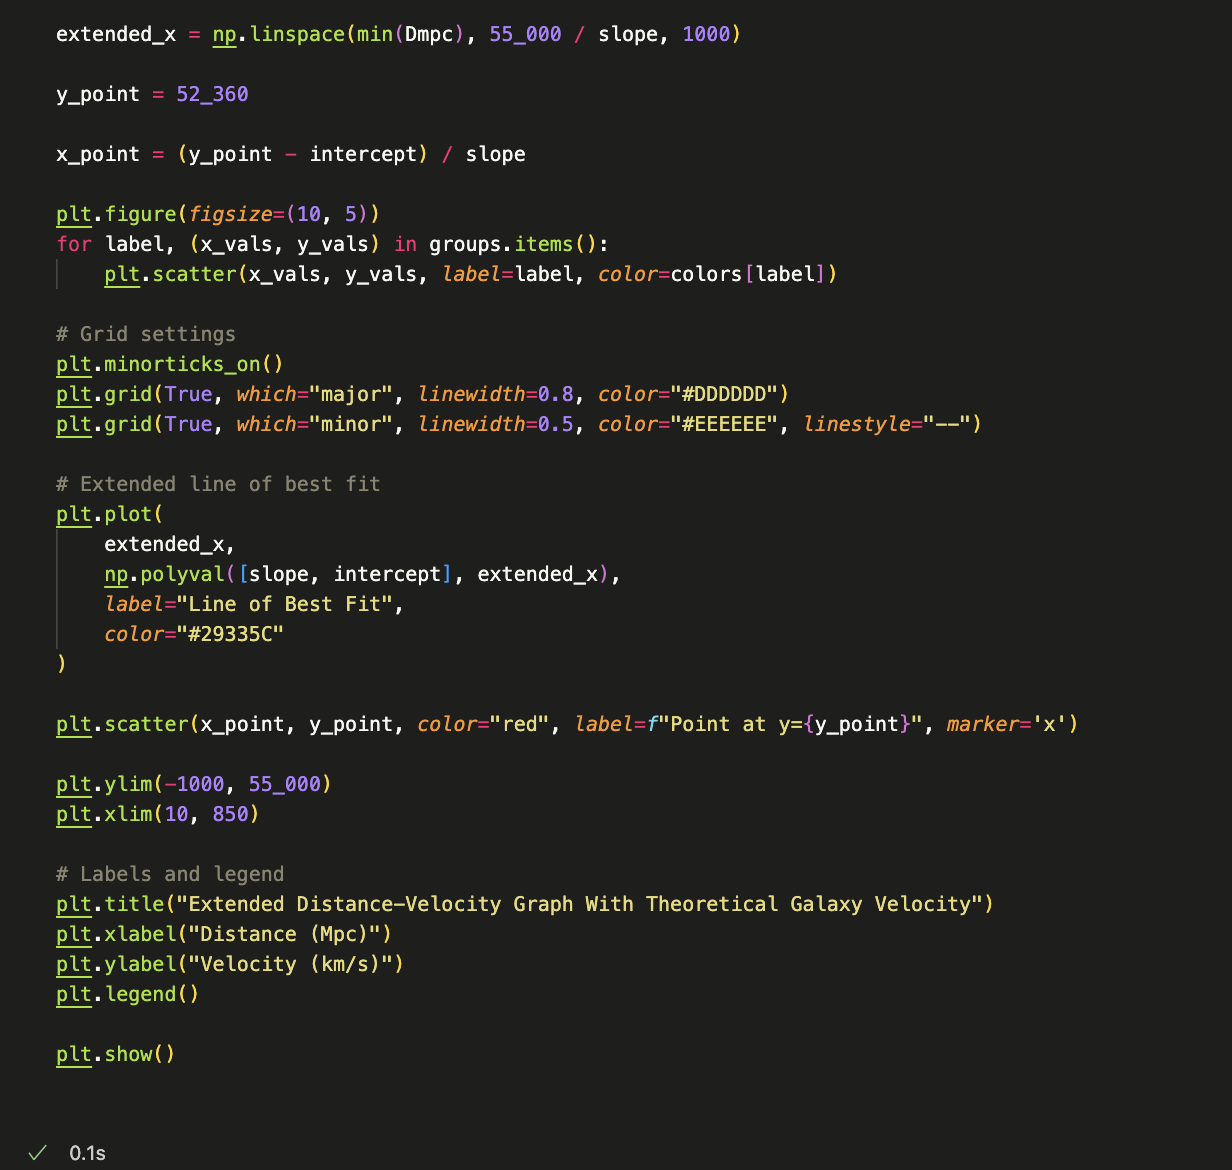
\includegraphics[width=\textwidth]{HUBBLEcode3.png}
    \caption{\centering Code for calculations (Python) Cont'd}
    \label{fig:code3}  
\end{figure}

\end{document}